\documentclass[]{article}
\usepackage{graphicx}
\usepackage{color}
\usepackage[utf8]{inputenc}

%opening
\title{Documentation Environment Store}
\author{Tim van Rossum, trvanrossum, 4246306}

\begin{document}

\maketitle

\section*{Size dialog}
At startup, a small GUI is shown that prompts the user to enter the amount of rows and columns the map has that they want to create. At the moment, for an existing map to be loaded in the map editor, the correct sizes of the map have to be entered before the map can be loaded. Figure one displays the size dialog:
\begin{center}
	\centering
	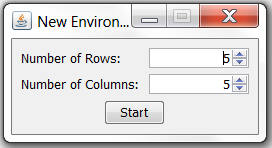
\includegraphics{SizeDialog.png}\\
	Figure 1: the size dialog
\end{center}
\section*{Map editor}
After specifying the amount of rows and columns the map should have, and clicking on the Start button, the map editor is launched. Figure 2 shows the environment store after launch, with a 5x5 map:
\begin{center}
	\centering
	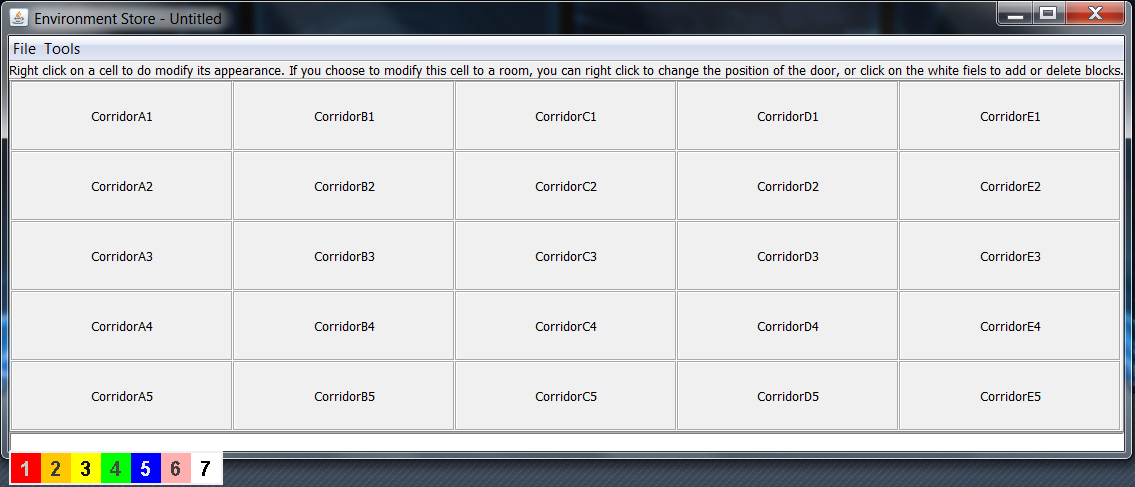
\includegraphics[scale=0.55]{MapEditor.png}\\
	Figure 2: the map editor with a 5x5 freshly created map
\end{center}
The map editor has many functionalities. The functionalities are detailed bit by bit in this documentation.
\section*{Editing a room}
Right click on any corridor (or any zone of the matrix for that matter), and the following drop down menu is shown:
\begin{center}
	\centering
	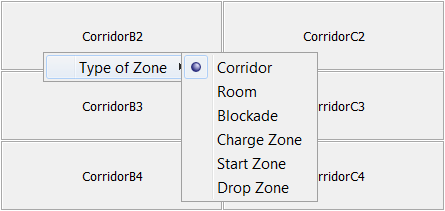
\includegraphics[scale=0.55]{DropDownMenuRoom.png}\\
	Figure 3: the drop down menu generated when a zone is right clicked
\end{center}
This allows a zone to be converted to any one of a corridor, a room, a blockade, a charge zone, a start zone, and a drop zone. The following figure shows the different appearances of the zones in the map editor:
\begin{center}
	\centering
	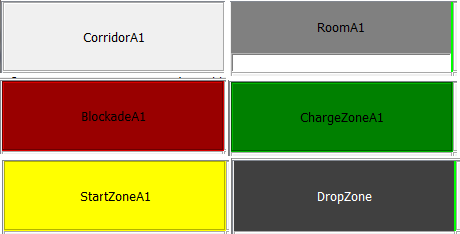
\includegraphics{DifferentRooms.png}\\
	Figure 4: the color palette at the bottom of the map editor
\end{center}
As can be seen, The room and drop zone contain a green border. This is to indicate which way the door to enter the room is faced. This is also editable. When right clicking on a certain room, the following drop down menu pops up:
\begin{center}
	\centering
	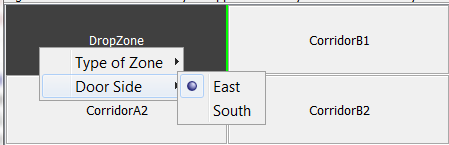
\includegraphics{DropDownMenuRoom2.png}\\
	Figure 5: the drop down menu generated when a room is right clicked
\end{center}
This drop down menu lists the directions the door can face while still being accessible. In this case, as it is the top left zone, only doors facing east or south are possible.
\section*{Editing a sequence}
Under the zones of the map editor is a white rectangle that contains the sequence for that map. This same rectangle is also present in the rooms that aren't drop zones. The rectangles are given here:
\begin{center}
	\centering
	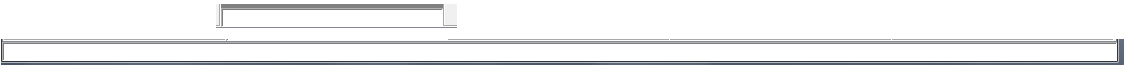
\includegraphics[scale=0.5]{SequenceEditor.png}\\
	Figure 6: The rectangle at the bottom of both the map editor and the rooms.
\end{center}
The rectangle in the rooms can be used to enter colors, which are then used in the blocks that are placed in that room. The rectangle under the zones can be used to enter the colors that make up the sequence that has to be completed for that map. To add colors, the color palette is useful.
\section*{Color palette}
At the bottom of the map editor is the color palette. A larger picture is given in figure 7:
\begin{center}
	\centering
	
\includegraphics{ColorPalette.png}\\
	Figure 7: the color palette at the bottom of the map editor
\end{center}
The color palette is used for adding blocks to rooms and the sequence to be completed in the map. When clicking on the box containing either the sequence of the map or the blocks in the room, the color palette is shown. It allows for the adding of colors by clicking on the respective colors on the palette, but colors can also be added by entering the respective numbers in the colors (pressing 1 adds a red block to the room or sequence, for example) and also by entering the first letter of the color (so pressing R adds a red block).
\section*{File menu}
The file menu contains not only the standard operations for exporting a created map to a file, so that it can be used later, but also a few other options. The drop down menu is as follows:
\begin{center}
	\centering
	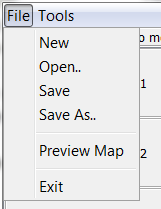
\includegraphics{DropDownFile.png}\\
	Figure 8: the drop down menu created when the 'File' menu item is clicked
\end{center}
The New-, Open...-, Save- and Save as...-options are the standard file operations and need no further explanation. However, as added functionality to the options, it is impossible to save a map not containing either a start- or drop zone, as well as a map not containing a block in its sequence, and saving an unsolvable map will give a warning describing what's wrong. The Exit-option also needs no further explanation. The Preview-option gives a preview of the created map, as how it would be rendered when used as an actual map for bots. For a non-edited 5x5 map, the preview looks as follows:
\begin{center}
	\centering
	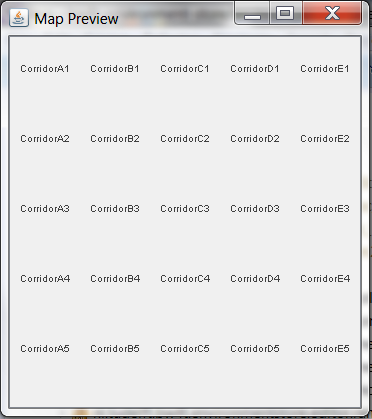
\includegraphics{Preview.png}\\
	Figure 9: The preview of a 5x5 non-edited map, with no blocks in the sequence
\end{center}
\section*{Tools menu}
The other drop down menu at the top of the map editor is the tools menu. This menu contains options to use several tools. The drop down menu is given here:
\begin{center}
	\centering
	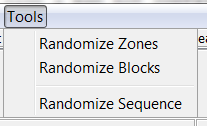
\includegraphics{DropDownTools.png}\\
	Figure 10: The drop down menu created when the 'Tools' menu item is clicked.
\end{center}
Clicking on the 'Randomize Zones' option creates a random map, based off a vanilla map with reclassification of rooms to blockades, charge zones or corridors, and with reclassifications of existing corridors to charge zones. The map is always solvable, given that all the blocks in the sequence are present in the map and no further changes are made to the map. The 'Randomize Blocks' option randomizes the blocks contained in every room according to parameters that the user has to specify. The interface for specifying the parameters is given here:
\begin{center}
	\centering
	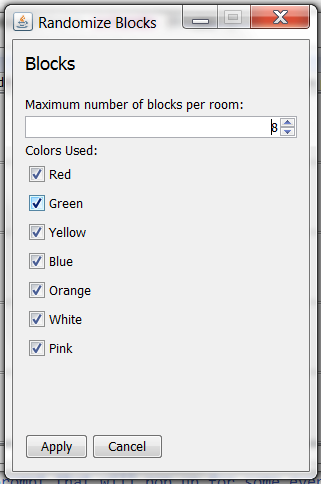
\includegraphics[scale=0.6]{MenuBlocks.png}\\
	Figure 11: The menu appearing when the randomize blocks option is clicked in the menu.
\end{center}
This interface allows the user to specify which block colors they want to be spawned, and also the max. amount of blocks in a room. The interface for random sequence generation is slightly different, and is as follows:
\begin{center}
	\centering
	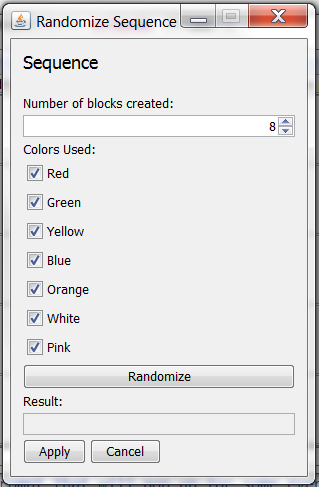
\includegraphics[scale=0.6]{MenuSeq.png}\\
	Figure 12: The menu appearing when the randomize blocks option is clicked in the menu.
\end{center}
The differences between this interface and the previous interface are the Randomize button and Result label, that  create and display resp. the random sequence, and the apply and cancel button which enter the sequence in the map or cancel the creation of the sequence, respectively.
\end{document}